\begin{center}
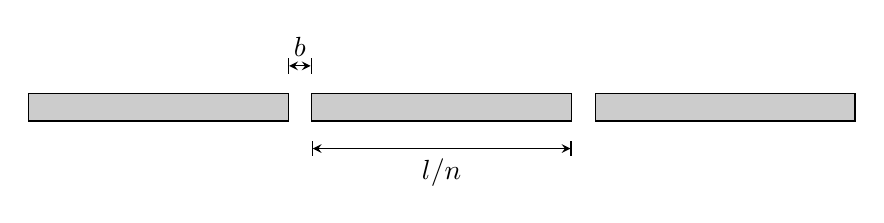
\begin{tikzpicture}[>=stealth]
 \foreach \x in {0,3.6,7.2} {
  \fill[gray!40] (\x,0) rectangle (\x+3.3,0.35);
  \draw (\x,0) rectangle (\x+3.3,0.35);
 }
 \draw[|<->|] (3.3,0.7) -- (3.6,0.7) node[midway, above] {$b$};
 \draw[|<->|] (3.6,-0.35) -- (6.9,-0.35) node[midway, below] {$l/n$};
\end{tikzpicture}
\end{center}

Annahmen: Die Schiene wird an einem heissen Sommertag bei $\vartheta_\mathrm{S} \approx \TSoO$ verlegt (sie liegt in der Sonne), die Lücken sind dabei fast geschlossen. Am eisigen Wintertag ist $\vartheta_\mathrm{W} \approx \TWiO$. Die Temperaturdifferenz ist
\begin{align}
 \Delta\vartheta &= \dTrF = \dTr
\end{align}
Mit $\alpha = \alStO$ (Kohlenstoffstahl, FoTaBe S.~190) zieht sich die Schiene insgesamt zusammen um
\begin{align}
 \Delta l &= \dlSF = \alSt\cdot\lSc\cdot\dTr = \dlS
\end{align}
Diese Verkürzung verteilt sich auf $n$ Lücken, von denen keine breiter als $b = \bLuO$ werden darf:
\begin{align}
 n &\geq \nLuF = \frac{\dlS}{\bLu} = \nLu
\end{align}
Man braucht also mindestens $\result{\nLaP{0}{2}}$ Lücken, d.\,h. etwa alle $\abLP{0}{2}$ eine. (Die alten Schienen waren tatsächlich nur einige Dutzend Meter lang.)
